\section{Results}\label{sec:results}

\subsection{Descriptive Evidence}

Table~\ref{tab:descriptives} summarizes the sample. Our analysis panel comprises 7,719 observations from 179 countries over 1970--2020. UNSC membership occurs in 6.1\% of country-years. The v3.1 stance score has mean 1.098 (SD = 1.142) and is concentrated at the upper end: 51.7\% of speeches receive the maximum score of $+2$, and only 4.1\% receive the minimum of $-2$. Real US aid averages \$172 million (2020 USD), with considerable right skew: the median is substantially below the mean, and 18.1\% of observations receive zero recorded aid.

\subsection{Construct Validation}

We assess convergent validity by correlating the v3.1 stance measure with two independently constructed behavioral indicators that were never used in measure development: UN voting agreement with the United States (\texttt{us\_agree}) and UN ideal point estimates (\texttt{ideal\_point}), both from Bailey, Strezhnev, and Voeten (2017). The correlations are small: $r(\text{stance}, \text{us\_agree}) = 0.085$ and $r(\text{stance}, \text{ideal\_point}) = 0.130$, based on 7,654 and 7,719 non-missing observations, respectively. These weak associations suggest either that diplomatic rhetoric and voting behavior capture distinct dimensions of alignment, or that the v3.1 measure captures something other than genuine geopolitical alignment with the United States. We return to this issue in Section~\ref{sec:discussion}.

\subsection{First Stage}

\begin{table}[htbp]
\centering
\caption{First Stage and Reduced Form Across Fixed-Effect Specifications}
\label{tab:fs_rf}
\begin{tabular}{lrrrrrr}
\toprule
& \multicolumn{3}{c}{\textbf{First Stage}} & \multicolumn{3}{c}{\textbf{Reduced Form}} \\
\cmidrule(lr){2-4} \cmidrule(lr){5-7}
Specification & Coef. & SE & $F$ & Coef. & SE & $p$ \\
\midrule
  None                 & +0.1450 & 0.5395 & 0.1 & -0.0747 & 0.0644 & 0.2458 \\
  Year FE              & +0.2694 & 0.5293 & 0.3 & -0.0684 & 0.0652 & 0.2946 \\
  Region FE            & +0.2794 & 0.4780 & 0.3 & -0.0721 & 0.0635 & 0.2559 \\
  Region x Year FE     & +0.4270 & 0.4604 & 0.9 & -0.0663 & 0.0645 & 0.3040 \\
  Country FE           & -0.1118 & 0.2215 & 0.3 & -0.1041 & 0.0558 & 0.0623 \\
  Country+Year FE      & -0.0575 & 0.2080 & 0.1 & -0.0996 & 0.0560 & 0.0754 \\
\midrule
\multicolumn{7}{p{0.85\textwidth}}{\footnotesize\textit{Note:} $N=7,719$, 179 countries, 1970--2020. Standard errors clustered at ISO3 level. First-stage $F=t^2$ on UNSC. Causal gate requires $F>10$ (Staiger and Stock, 1997). KW2006 specifications are Region FE and Region~x~Year~FE. No specification meets the $F>10$ threshold.}\\
\end{tabular}
\end{table}


Table~\ref{tab:fs_rf} reports the first-stage and reduced-form estimates across six fixed-effect specifications. Our key findings are threefold.

First, \textbf{the causal gate is closed} in every specification. Under country--year FE (column 6), the UNSC coefficient on $\log(1+\text{Aid})$ is $\hat{\beta} = -0.058$ (SE = 0.208), yielding $F = 0.1$. The point estimate is close to zero and statistically indistinguishable from it ($p = 0.782$). Adding GDP per capita, population, and trade openness as controls produces $\hat{\beta} = -0.136$ (SE = 0.233, $F = 0.3$). No specification approaches the $F>10$ threshold required for reliable 2SLS inference.

Second, \textbf{the Kuziemko--Werker (2006) specification does not rescue the instrument.} Under region--year FE (column 4), the UNSC coefficient is $\hat{\beta} = +0.427$ (SE = 0.460), but the $F$-statistic is only 0.9 ($p = 0.354$). The coefficient is positive, as predicted, but the statistical uncertainty is too large to reject the null of no first-stage relationship. This is a critical finding: even the specification closest to the original Kuziemko--Werker design fails to produce a significant first stage in our data.

Third, \textbf{the first stage is not sensitive to sample composition.} Across four named samples (all available, verified complete, original untruncated, and validation available), the $F$-statistic under country--year FE never exceeds 0.1. The sign of the coefficient varies across specifications but is never statistically significant.

\subsection{Reduced Form}

The reduced form is consistently negative across specifications. Under country--year FE, the UNSC effect on stance is $\hat{\delta} = -0.100$ (SE = 0.056, $p = 0.075$). This estimate is directionally stable: in five of six FE specifications, the point estimate is negative, ranging from $-0.066$ (region--year FE) to $-0.104$ (country FE). The $p$-value is at or above conventional significance thresholds in all specifications, with the smallest being $p = 0.062$ under country FE.

The negative sign, while not statistically significant, runs counter to the ``material power buys allegiance'' hypothesis: if anything, UNSC members express \emph{less} pro-US sentiment in their General Debate speeches than non-members. The magnitude is small---approximately 0.09 standard deviations of the stance measure---making it difficult to distinguish from statistical noise even with 7,719 observations.

\subsection{Event Study}

\begin{figure}[htbp]
\centering
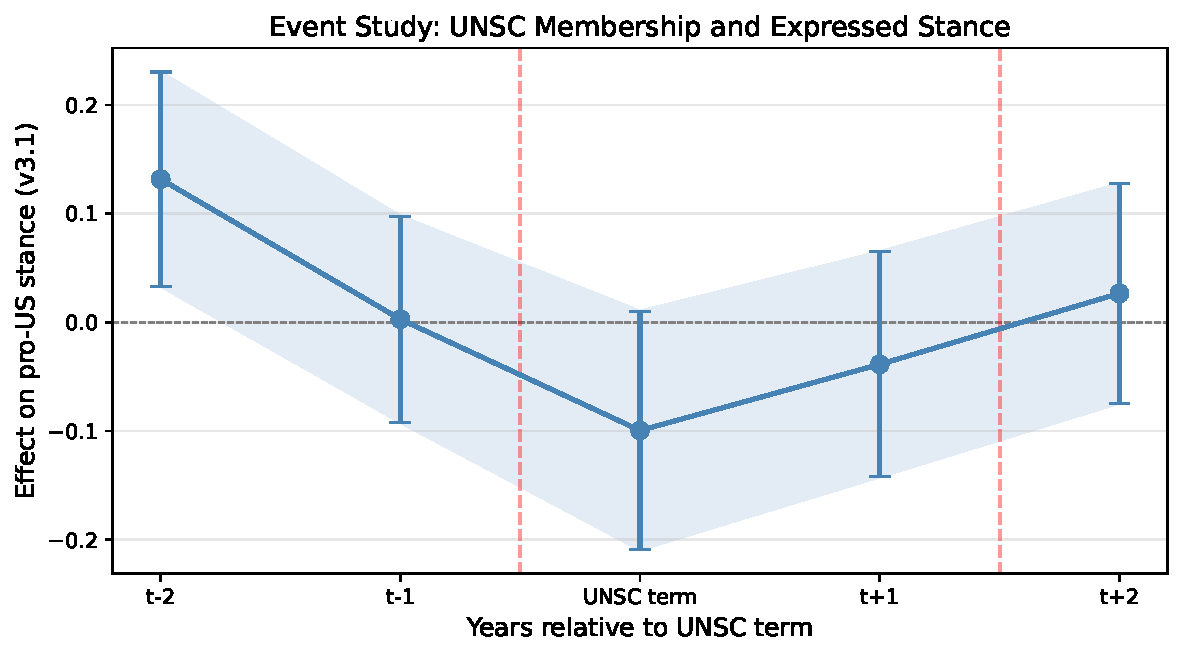
\includegraphics[width=0.85\textwidth]{../../figures/main/event_study.pdf}
\caption{Event study: UNSC membership and expressed stance. Points are coefficient estimates from regressions of stance on UNSC indicators at leads $t-2$ and $t-1$, the contemporaneous UNSC term, and lags $t+1$ and $t+2$. All specifications include country and year fixed effects. Error bars show 95\% confidence intervals with standard errors clustered at the ISO3 level. The red dashed lines mark the UNSC term boundaries.}
\label{fig:event_study}
\end{figure}

Figure~\ref{fig:event_study} displays leads and lags around the two-year UNSC term. The lead-2 coefficient is marginally positive ($+0.132$, SE = 0.050, $p = 0.009$), indicating that two years before their UNSC term, countries express slightly \emph{more} pro-US sentiment. The lead-1 coefficient is essentially zero ($+0.003$, $p = 0.955$), the contemporaneous UNSC coefficient is negative ($-0.100$, $p = 0.075$), and both lag coefficients are small and statistically insignificant (lag-1: $-0.039$, $p = 0.464$; lag-2: $+0.027$, $p = 0.606$).

The lead-2 pattern is consistent with pre-election campaigning: countries seeking a UNSC seat may intensify diplomatic outreach to major powers, including the US, two years before their term begins. However, the absence of systematic pre-trends (lead-1 is zero) and the absence of post-term effects (both lags are null) argue against a strong causal interpretation. The event study broadly supports the null reduced-form finding: UNSC membership is not associated with systematic changes in expressed US stance.

\subsection{Causal Gate Assessment}

The causal gate is closed. The first-stage $F$-statistic under the preferred specification is 0.1, far below the pre-registered threshold of 10. We do not report 2SLS estimates. Following our pre-registered analysis plan, the paper centers on the reduced form, event-study estimates, and robustness checks. The null finding does not reflect a failure of our analysis but rather a substantive empirical result: UNSC membership, in this data, does not predict US aid receipts within countries over time, and the reduced-form effect on speech stance is null.
